\PassOptionsToPackage{unicode=true}{hyperref} % options for packages loaded elsewhere
\PassOptionsToPackage{hyphens}{url}
\PassOptionsToPackage{dvipsnames,svgnames*,x11names*}{xcolor}
%
\documentclass[]{article}
\usepackage{lmodern}
\usepackage{amssymb,amsmath}
\usepackage{ifxetex,ifluatex}
\usepackage{fixltx2e} % provides \textsubscript
\ifnum 0\ifxetex 1\fi\ifluatex 1\fi=0 % if pdftex
  \usepackage[T1]{fontenc}
  \usepackage[utf8]{inputenc}
  \usepackage{textcomp} % provides euro and other symbols
\else % if luatex or xelatex
  \usepackage{unicode-math}
  \defaultfontfeatures{Ligatures=TeX,Scale=MatchLowercase}
\fi
% use upquote if available, for straight quotes in verbatim environments
\IfFileExists{upquote.sty}{\usepackage{upquote}}{}
% use microtype if available
\IfFileExists{microtype.sty}{%
\usepackage[]{microtype}
\UseMicrotypeSet[protrusion]{basicmath} % disable protrusion for tt fonts
}{}
\IfFileExists{parskip.sty}{%
\usepackage{parskip}
}{% else
\setlength{\parindent}{0pt}
\setlength{\parskip}{6pt plus 2pt minus 1pt}
}
\usepackage{xcolor}
\usepackage{hyperref}
\hypersetup{
            pdftitle={Module 8: Solutions to Recommended Exercises},
            pdfauthor={Emma Skarstein, Michail Spitieris, Stefanie Muff; Department of Mathematical Sciences, NTNU},
            colorlinks=true,
            linkcolor=Maroon,
            filecolor=Maroon,
            citecolor=Blue,
            urlcolor=blue,
            breaklinks=true}
\urlstyle{same}  % don't use monospace font for urls
\usepackage[margin=1in]{geometry}
\usepackage{color}
\usepackage{fancyvrb}
\newcommand{\VerbBar}{|}
\newcommand{\VERB}{\Verb[commandchars=\\\{\}]}
\DefineVerbatimEnvironment{Highlighting}{Verbatim}{commandchars=\\\{\}}
% Add ',fontsize=\small' for more characters per line
\usepackage{framed}
\definecolor{shadecolor}{RGB}{248,248,248}
\newenvironment{Shaded}{\begin{snugshade}}{\end{snugshade}}
\newcommand{\AlertTok}[1]{\textcolor[rgb]{0.94,0.16,0.16}{#1}}
\newcommand{\AnnotationTok}[1]{\textcolor[rgb]{0.56,0.35,0.01}{\textbf{\textit{#1}}}}
\newcommand{\AttributeTok}[1]{\textcolor[rgb]{0.77,0.63,0.00}{#1}}
\newcommand{\BaseNTok}[1]{\textcolor[rgb]{0.00,0.00,0.81}{#1}}
\newcommand{\BuiltInTok}[1]{#1}
\newcommand{\CharTok}[1]{\textcolor[rgb]{0.31,0.60,0.02}{#1}}
\newcommand{\CommentTok}[1]{\textcolor[rgb]{0.56,0.35,0.01}{\textit{#1}}}
\newcommand{\CommentVarTok}[1]{\textcolor[rgb]{0.56,0.35,0.01}{\textbf{\textit{#1}}}}
\newcommand{\ConstantTok}[1]{\textcolor[rgb]{0.00,0.00,0.00}{#1}}
\newcommand{\ControlFlowTok}[1]{\textcolor[rgb]{0.13,0.29,0.53}{\textbf{#1}}}
\newcommand{\DataTypeTok}[1]{\textcolor[rgb]{0.13,0.29,0.53}{#1}}
\newcommand{\DecValTok}[1]{\textcolor[rgb]{0.00,0.00,0.81}{#1}}
\newcommand{\DocumentationTok}[1]{\textcolor[rgb]{0.56,0.35,0.01}{\textbf{\textit{#1}}}}
\newcommand{\ErrorTok}[1]{\textcolor[rgb]{0.64,0.00,0.00}{\textbf{#1}}}
\newcommand{\ExtensionTok}[1]{#1}
\newcommand{\FloatTok}[1]{\textcolor[rgb]{0.00,0.00,0.81}{#1}}
\newcommand{\FunctionTok}[1]{\textcolor[rgb]{0.00,0.00,0.00}{#1}}
\newcommand{\ImportTok}[1]{#1}
\newcommand{\InformationTok}[1]{\textcolor[rgb]{0.56,0.35,0.01}{\textbf{\textit{#1}}}}
\newcommand{\KeywordTok}[1]{\textcolor[rgb]{0.13,0.29,0.53}{\textbf{#1}}}
\newcommand{\NormalTok}[1]{#1}
\newcommand{\OperatorTok}[1]{\textcolor[rgb]{0.81,0.36,0.00}{\textbf{#1}}}
\newcommand{\OtherTok}[1]{\textcolor[rgb]{0.56,0.35,0.01}{#1}}
\newcommand{\PreprocessorTok}[1]{\textcolor[rgb]{0.56,0.35,0.01}{\textit{#1}}}
\newcommand{\RegionMarkerTok}[1]{#1}
\newcommand{\SpecialCharTok}[1]{\textcolor[rgb]{0.00,0.00,0.00}{#1}}
\newcommand{\SpecialStringTok}[1]{\textcolor[rgb]{0.31,0.60,0.02}{#1}}
\newcommand{\StringTok}[1]{\textcolor[rgb]{0.31,0.60,0.02}{#1}}
\newcommand{\VariableTok}[1]{\textcolor[rgb]{0.00,0.00,0.00}{#1}}
\newcommand{\VerbatimStringTok}[1]{\textcolor[rgb]{0.31,0.60,0.02}{#1}}
\newcommand{\WarningTok}[1]{\textcolor[rgb]{0.56,0.35,0.01}{\textbf{\textit{#1}}}}
\usepackage{graphicx,grffile}
\makeatletter
\def\maxwidth{\ifdim\Gin@nat@width>\linewidth\linewidth\else\Gin@nat@width\fi}
\def\maxheight{\ifdim\Gin@nat@height>\textheight\textheight\else\Gin@nat@height\fi}
\makeatother
% Scale images if necessary, so that they will not overflow the page
% margins by default, and it is still possible to overwrite the defaults
% using explicit options in \includegraphics[width, height, ...]{}
\setkeys{Gin}{width=\maxwidth,height=\maxheight,keepaspectratio}
\setlength{\emergencystretch}{3em}  % prevent overfull lines
\providecommand{\tightlist}{%
  \setlength{\itemsep}{0pt}\setlength{\parskip}{0pt}}
\setcounter{secnumdepth}{0}
% Redefines (sub)paragraphs to behave more like sections
\ifx\paragraph\undefined\else
\let\oldparagraph\paragraph
\renewcommand{\paragraph}[1]{\oldparagraph{#1}\mbox{}}
\fi
\ifx\subparagraph\undefined\else
\let\oldsubparagraph\subparagraph
\renewcommand{\subparagraph}[1]{\oldsubparagraph{#1}\mbox{}}
\fi

% set default figure placement to htbp
\makeatletter
\def\fps@figure{htbp}
\makeatother

\usepackage{etoolbox}
\makeatletter
\providecommand{\subtitle}[1]{% add subtitle to \maketitle
  \apptocmd{\@title}{\par {\large #1 \par}}{}{}
}
\makeatother

\title{Module 8: Solutions to Recommended Exercises}
\providecommand{\subtitle}[1]{}
\subtitle{TMA4268 Statistical Learning V2021}
\author{Emma Skarstein, Michail Spitieris, Stefanie Muff \and Department of Mathematical Sciences, NTNU}
\date{March 9, 2021}

\begin{document}
\maketitle

\begin{center}\rule{0.5\linewidth}{0.5pt}\end{center}

\hypertarget{problem-1-theoretical}{%
\subsection{Problem 1 -- Theoretical}\label{problem-1-theoretical}}

\begin{enumerate}
\def\labelenumi{\alph{enumi})}
\item
\end{enumerate}

\begin{enumerate}
\def\labelenumi{\arabic{enumi}.}
\item
  \emph{Recursive binary splitting}: We find the best single
  partitioning of the data such that the reduction of RSS is the
  greatest. This process is applied sequencially to each of the split
  parts until a predefined minimum number of leave observation is
  reached.
\item
  \emph{Cost complexity pruning} of the large tree from previoius step,
  in order to obtain a sequence of best trees as a function of a
  parameter \(\alpha\). Each value of \(\alpha\) corresponds to a
  subtree that minimize the following equation (several \(\alpha\)s for
  the same tree):
\end{enumerate}

\[\sum_{m=1}^{|T|}\sum_{i:x_i\in R_m}(y_i - \hat y_{R_m})^2 + \alpha |T|,\]

where \(|T|\) is the numb er of terminal nodes.

\begin{enumerate}
\def\labelenumi{\arabic{enumi}.}
\setcounter{enumi}{2}
\tightlist
\item
  \emph{\(K\)-fold cross-validation} to choose \(\alpha\). For each
  fold:
\end{enumerate}

\begin{itemize}
\tightlist
\item
  Repeat Steps 1 and 2 on all but the kth folds of the training data.
\item
  Evaluate the mean squared prediction on the data in the left-out kth
  fold, as a function of \(\alpha\).
\item
  Average the results for each value of \(\alpha\) and choose \(\alpha\)
  to minimize the average error.
\end{itemize}

\begin{enumerate}
\def\labelenumi{\arabic{enumi}.}
\setcounter{enumi}{3}
\tightlist
\item
  Return the subtree from Step 2 that corresponds to the chosen value of
  \(\alpha.\)
\end{enumerate}

For a \textbf{classification} tree we replace RSS with Gini index or
entropy.

\begin{enumerate}
\def\labelenumi{\alph{enumi})}
\setcounter{enumi}{1}
\item
\end{enumerate}

\(\color{green}{\text{Advantages}}\)

\begin{itemize}
\item
  Very easy to explain
\item
  Can be displayed graphically
\item
  Can handle both quantitative and qualitative predictors without the
  need to create dummy variables
\end{itemize}

\(\color{red}{\text{Disadvantages}}\)

\begin{itemize}
\item
  The predictive accuracy is usualy not very high
\item
  They are non-robust. That is a small change in the data can cause a
  large change in the estimated tree
\end{itemize}

\begin{enumerate}
\def\labelenumi{\alph{enumi})}
\setcounter{enumi}{2}
\item
\end{enumerate}

Decision trees suffer from high variance. Recall that if we have \(B\)
\(i.i.d\) observations of a random variable \(X\) with the same mean and
variance \(\sigma^2.\) We calculate the mean
\(\bar{X} = \frac{1}{B} \sum_{b=1}^B X_b,\) and the variance of the mean
is \(\text{Var}(\bar{X}) = \frac{\sigma^2}{B}.\) That is by averaging we
get reduced variance.

For decision trees, if we have \(B\) training sets, we could estimate
\(\hat{f}_1({\boldsymbol x}),\hat{f}_2({\boldsymbol x}),\ldots, \hat{f}_B({\boldsymbol x})\)
and average them as
\[\hat{f}_{avg}({\boldsymbol x})=\frac{1}{B}\sum_{b=1}^B \hat{f}_b({\boldsymbol x}) \ .\]
However we do not have many data independent data sets, and we
bootstraping to create \(B\) datasets. These datasets are however not
completely independent and the reduction in variance is therefore not as
large as for independent training sets.

To make the different trees that are built from each bootstrapped
dataset more different, random forests use a random subset of the
predictors to split the tree into new branches at each step. This
decorrelates the different trees that are built from the \(B\)
bootstrapped datasets, and consequently reduces variance.

\begin{enumerate}
\def\labelenumi{\alph{enumi})}
\setcounter{enumi}{3}
\item
  An OOB is the set of observations that were not chosen to be in a
  specific bootstrap sample. From RecEx5-Problem 4c we have that on
  average \(1-0.632 = 0.368\) are included in the OOB sample.
\item
\end{enumerate}

\textbf{Variable importance based on node impurity}

\textbf{Regression Trees}: The total amount that the RSS is decreased
due to splits of each predictor, averaged over the B trees.

\textbf{Classification Trees}: The importance is the mean decrease (over
all B trees) in the Gini index by splits of a predictor.

\textbf{Variable importance based on randomization}

This measure is based on how much the predictive accuracy (MSE or gini
indiex) is decreased when the variable is replaced by a permuted version
of it. You find a drawing
\href{https://github.com/stefaniemuff/statlearning/blob/master/8Trees/M8_variableImportanceRandomization.pdf}{here}.

\hypertarget{problem-2-regression-book-ex.-8}{%
\subsection{Problem 2 -- Regression (Book Ex.
8)}\label{problem-2-regression-book-ex.-8}}

\begin{enumerate}
\def\labelenumi{\alph{enumi})}
\item
\end{enumerate}

\begin{Shaded}
\begin{Highlighting}[]
\KeywordTok{library}\NormalTok{(ISLR)}
\KeywordTok{data}\NormalTok{(}\StringTok{"Carseats"}\NormalTok{)}
\KeywordTok{set.seed}\NormalTok{(}\DecValTok{4268}\NormalTok{)}
\NormalTok{n =}\StringTok{ }\KeywordTok{nrow}\NormalTok{(Carseats)}
\NormalTok{train =}\StringTok{ }\KeywordTok{sample}\NormalTok{(}\DecValTok{1}\OperatorTok{:}\NormalTok{n, }\FloatTok{0.7} \OperatorTok{*}\StringTok{ }\KeywordTok{nrow}\NormalTok{(Carseats), }\DataTypeTok{replace =}\NormalTok{ F)}
\NormalTok{test =}\StringTok{ }\NormalTok{(}\DecValTok{1}\OperatorTok{:}\NormalTok{n)[}\OperatorTok{-}\NormalTok{train]}
\NormalTok{Carseats.train =}\StringTok{ }\NormalTok{Carseats[train, ]}
\NormalTok{Carseats.test =}\StringTok{ }\NormalTok{Carseats[}\OperatorTok{-}\NormalTok{train, ]}
\end{Highlighting}
\end{Shaded}

\begin{enumerate}
\def\labelenumi{\alph{enumi})}
\setcounter{enumi}{1}
\item
\end{enumerate}

\begin{Shaded}
\begin{Highlighting}[]
\KeywordTok{library}\NormalTok{(tree)}
\NormalTok{tree.mod =}\StringTok{ }\KeywordTok{tree}\NormalTok{(Sales }\OperatorTok{~}\StringTok{ }\NormalTok{., Carseats, }\DataTypeTok{subset =}\NormalTok{ train)}
\KeywordTok{summary}\NormalTok{(tree.mod)}
\end{Highlighting}
\end{Shaded}

\begin{verbatim}
## 
## Regression tree:
## tree(formula = Sales ~ ., data = Carseats, subset = train)
## Variables actually used in tree construction:
## [1] "ShelveLoc"   "Price"       "Age"         "Income"      "CompPrice"  
## [6] "Population"  "Advertising" "Education"  
## Number of terminal nodes:  18 
## Residual mean deviance:  2.609 = 683.6 / 262 
## Distribution of residuals:
##     Min.  1st Qu.   Median     Mean  3rd Qu.     Max. 
## -3.74000 -1.12400 -0.06522  0.00000  1.06800  4.47200
\end{verbatim}

\begin{Shaded}
\begin{Highlighting}[]
\KeywordTok{plot}\NormalTok{(tree.mod)}
\KeywordTok{text}\NormalTok{(tree.mod, }\DataTypeTok{pretty =} \DecValTok{0}\NormalTok{)}
\end{Highlighting}
\end{Shaded}

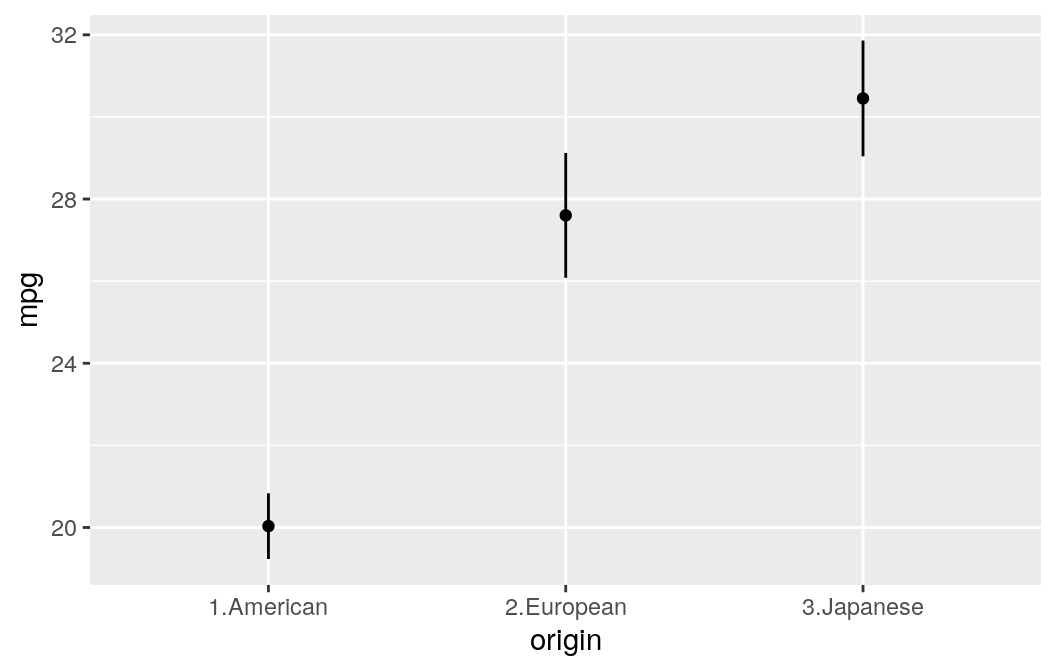
\includegraphics[width=0.7\linewidth]{RecEx8-sol_files/figure-latex/unnamed-chunk-3-1}

\begin{Shaded}
\begin{Highlighting}[]
\NormalTok{yhat =}\StringTok{ }\KeywordTok{predict}\NormalTok{(tree.mod, }\DataTypeTok{newdata =}\NormalTok{ Carseats.test)}
\NormalTok{mse =}\StringTok{ }\KeywordTok{mean}\NormalTok{((yhat }\OperatorTok{-}\StringTok{ }\NormalTok{Carseats.test}\OperatorTok{$}\NormalTok{Sales)}\OperatorTok{^}\DecValTok{2}\NormalTok{)}
\NormalTok{mse}
\end{Highlighting}
\end{Shaded}

\begin{verbatim}
## [1] 4.585249
\end{verbatim}

\begin{enumerate}
\def\labelenumi{\alph{enumi})}
\setcounter{enumi}{2}
\item
\end{enumerate}

\begin{Shaded}
\begin{Highlighting}[]
\KeywordTok{set.seed}\NormalTok{(}\DecValTok{4268}\NormalTok{)}
\NormalTok{cv.Carseats =}\StringTok{ }\KeywordTok{cv.tree}\NormalTok{(tree.mod)}
\NormalTok{tree.min =}\StringTok{ }\KeywordTok{which.min}\NormalTok{(cv.Carseats}\OperatorTok{$}\NormalTok{dev)}
\NormalTok{best =}\StringTok{ }\NormalTok{cv.Carseats}\OperatorTok{$}\NormalTok{size[tree.min]}
\KeywordTok{plot}\NormalTok{(cv.Carseats}\OperatorTok{$}\NormalTok{size, cv.Carseats}\OperatorTok{$}\NormalTok{dev, }\DataTypeTok{type =} \StringTok{"b"}\NormalTok{)}
\KeywordTok{points}\NormalTok{(cv.Carseats}\OperatorTok{$}\NormalTok{size[tree.min], cv.Carseats}\OperatorTok{$}\NormalTok{dev[tree.min], }\DataTypeTok{col =} \StringTok{"red"}\NormalTok{, }\DataTypeTok{pch =} \DecValTok{20}\NormalTok{)}
\end{Highlighting}
\end{Shaded}

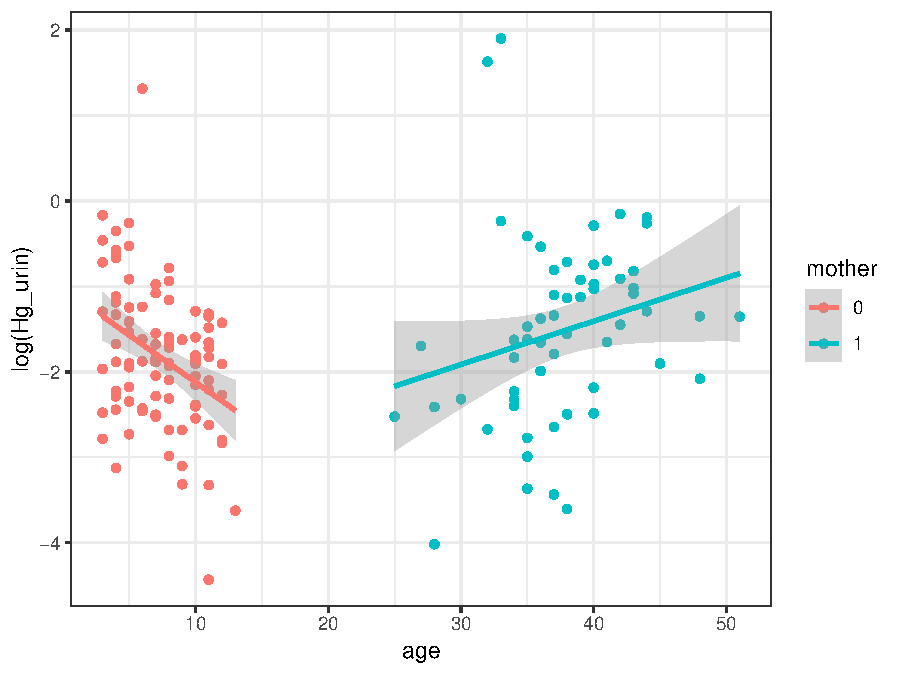
\includegraphics{RecEx8-sol_files/figure-latex/unnamed-chunk-4-1.pdf}

We see that trees with sizes 11, 12, 16 and 17 have similar deviance
values. We should ideally choose the tree of size 11 as it gives the
simpler tree.

\begin{Shaded}
\begin{Highlighting}[]
\NormalTok{pr.tree =}\StringTok{ }\KeywordTok{prune.tree}\NormalTok{(tree.mod, }\DataTypeTok{best =} \DecValTok{11}\NormalTok{)}
\KeywordTok{plot}\NormalTok{(pr.tree)}
\KeywordTok{text}\NormalTok{(pr.tree, }\DataTypeTok{pretty =} \DecValTok{0}\NormalTok{)}
\end{Highlighting}
\end{Shaded}

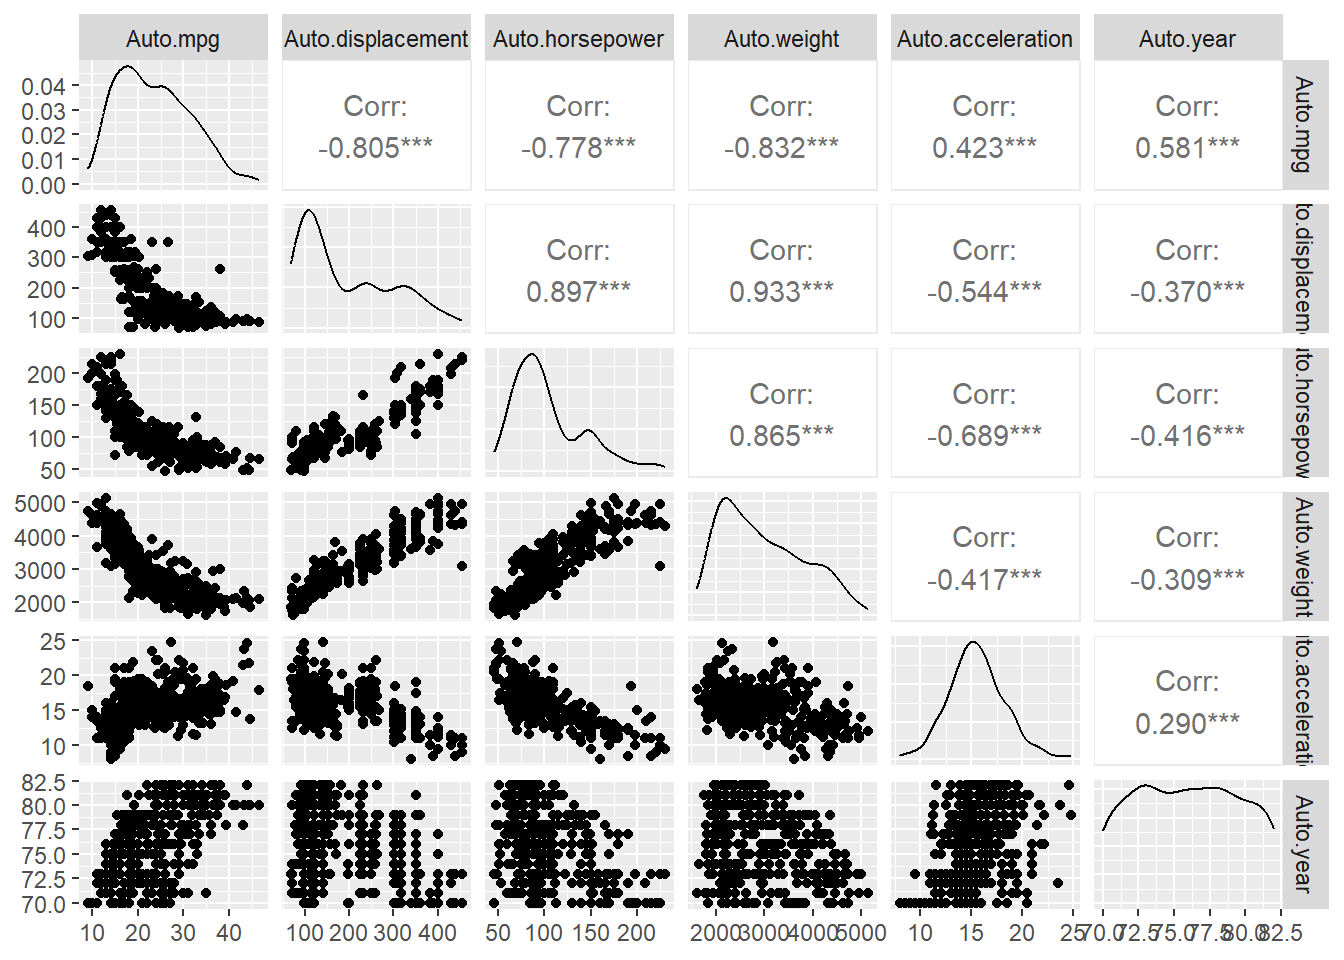
\includegraphics[width=0.7\linewidth]{RecEx8-sol_files/figure-latex/unnamed-chunk-5-1}

\begin{Shaded}
\begin{Highlighting}[]
\NormalTok{yhat =}\StringTok{ }\KeywordTok{predict}\NormalTok{(pr.tree, }\DataTypeTok{newdata =}\NormalTok{ Carseats.test)}
\NormalTok{mse =}\StringTok{ }\KeywordTok{mean}\NormalTok{((yhat }\OperatorTok{-}\StringTok{ }\NormalTok{Carseats.test}\OperatorTok{$}\NormalTok{Sales)}\OperatorTok{^}\DecValTok{2}\NormalTok{)}
\NormalTok{mse}
\end{Highlighting}
\end{Shaded}

\begin{verbatim}
## [1] 4.378499
\end{verbatim}

There is a slight reduction in MSE for the pruned tree with 11 leaves.

\begin{enumerate}
\def\labelenumi{\alph{enumi})}
\setcounter{enumi}{3}
\item
\end{enumerate}

\begin{Shaded}
\begin{Highlighting}[]
\KeywordTok{library}\NormalTok{(randomForest)}
\KeywordTok{dim}\NormalTok{(Carseats)}
\end{Highlighting}
\end{Shaded}

\begin{verbatim}
## [1] 400  11
\end{verbatim}

\begin{Shaded}
\begin{Highlighting}[]
\NormalTok{bag.Carseats =}\StringTok{ }\KeywordTok{randomForest}\NormalTok{(Sales }\OperatorTok{~}\StringTok{ }\NormalTok{., Carseats.train, }\DataTypeTok{mtry =} \KeywordTok{ncol}\NormalTok{(Carseats) }\OperatorTok{-}\StringTok{ }\DecValTok{1}\NormalTok{, }
    \DataTypeTok{ntree =} \DecValTok{500}\NormalTok{, }\DataTypeTok{importance =} \OtherTok{TRUE}\NormalTok{)}
\NormalTok{yhat.bag =}\StringTok{ }\KeywordTok{predict}\NormalTok{(bag.Carseats, }\DataTypeTok{newdata =}\NormalTok{ Carseats.test)}
\NormalTok{mse.bag =}\StringTok{ }\KeywordTok{mean}\NormalTok{((yhat.bag }\OperatorTok{-}\StringTok{ }\NormalTok{Carseats.test}\OperatorTok{$}\NormalTok{Sales)}\OperatorTok{^}\DecValTok{2}\NormalTok{)}
\NormalTok{mse.bag}
\end{Highlighting}
\end{Shaded}

\begin{verbatim}
## [1] 2.122958
\end{verbatim}

Bagging decreases the test MSE significantly to 2.12. From the
importance plots we might conclude that \texttt{Price}and
\texttt{ShelveLoc} are the most important Variables.

\begin{Shaded}
\begin{Highlighting}[]
\KeywordTok{importance}\NormalTok{(bag.Carseats)}
\end{Highlighting}
\end{Shaded}

\begin{verbatim}
##               %IncMSE IncNodePurity
## CompPrice   26.803869    218.740455
## Income      10.284817    127.447480
## Advertising 25.795425    196.438893
## Population   6.084270     92.149065
## Price       67.791459    667.696518
## ShelveLoc   75.485534    734.902022
## Age         24.961130    229.491494
## Education    3.423565     64.510742
## Urban       -1.373635      9.423406
## US           3.141449     10.105870
\end{verbatim}

\begin{Shaded}
\begin{Highlighting}[]
\KeywordTok{varImpPlot}\NormalTok{(bag.Carseats)}
\end{Highlighting}
\end{Shaded}

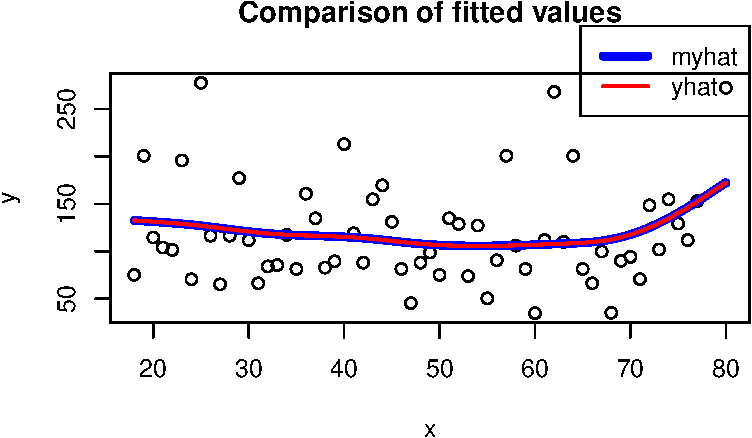
\includegraphics[width=0.8\linewidth]{RecEx8-sol_files/figure-latex/unnamed-chunk-8-1}

\begin{enumerate}
\def\labelenumi{\alph{enumi})}
\setcounter{enumi}{4}
\item
\end{enumerate}

\begin{Shaded}
\begin{Highlighting}[]
\NormalTok{rf.Carseats =}\StringTok{ }\KeywordTok{randomForest}\NormalTok{(Sales }\OperatorTok{~}\StringTok{ }\NormalTok{., }\DataTypeTok{data =}\NormalTok{ Carseats.train, }\DataTypeTok{mtry =} \DecValTok{3}\NormalTok{, }\DataTypeTok{ntree =} \DecValTok{500}\NormalTok{, }
    \DataTypeTok{importance =} \OtherTok{TRUE}\NormalTok{)}
\NormalTok{yhat.rf =}\StringTok{ }\KeywordTok{predict}\NormalTok{(rf.Carseats, }\DataTypeTok{newdata =}\NormalTok{ Carseats.test)}
\NormalTok{mse_forest <-}\StringTok{ }\KeywordTok{mean}\NormalTok{((yhat.rf }\OperatorTok{-}\StringTok{ }\NormalTok{Carseats.test}\OperatorTok{$}\NormalTok{Sales)}\OperatorTok{^}\DecValTok{2}\NormalTok{)}
\NormalTok{mse_forest}
\end{Highlighting}
\end{Shaded}

\begin{verbatim}
## [1] 2.25397
\end{verbatim}

We use \(p/3 = 10/3 \approx 3\) trees, and we obtain an MSE of 2.25
which is slightly larger than Bagging MSE. The two most important
Variables are again \texttt{Price}and \texttt{ShelveLoc}.

\begin{Shaded}
\begin{Highlighting}[]
\KeywordTok{importance}\NormalTok{(rf.Carseats)}
\end{Highlighting}
\end{Shaded}

\begin{verbatim}
##               %IncMSE IncNodePurity
## CompPrice   15.789484     211.79213
## Income       5.415374     174.79625
## Advertising 18.402600     210.47149
## Population   1.076874     148.09993
## Price       45.548596     577.68865
## ShelveLoc   47.810006     549.62278
## Age         15.936114     241.99130
## Education    3.275725     104.89503
## Urban       -1.646580      19.63668
## US           5.427599      36.45647
\end{verbatim}

\begin{Shaded}
\begin{Highlighting}[]
\KeywordTok{varImpPlot}\NormalTok{(rf.Carseats)}
\end{Highlighting}
\end{Shaded}

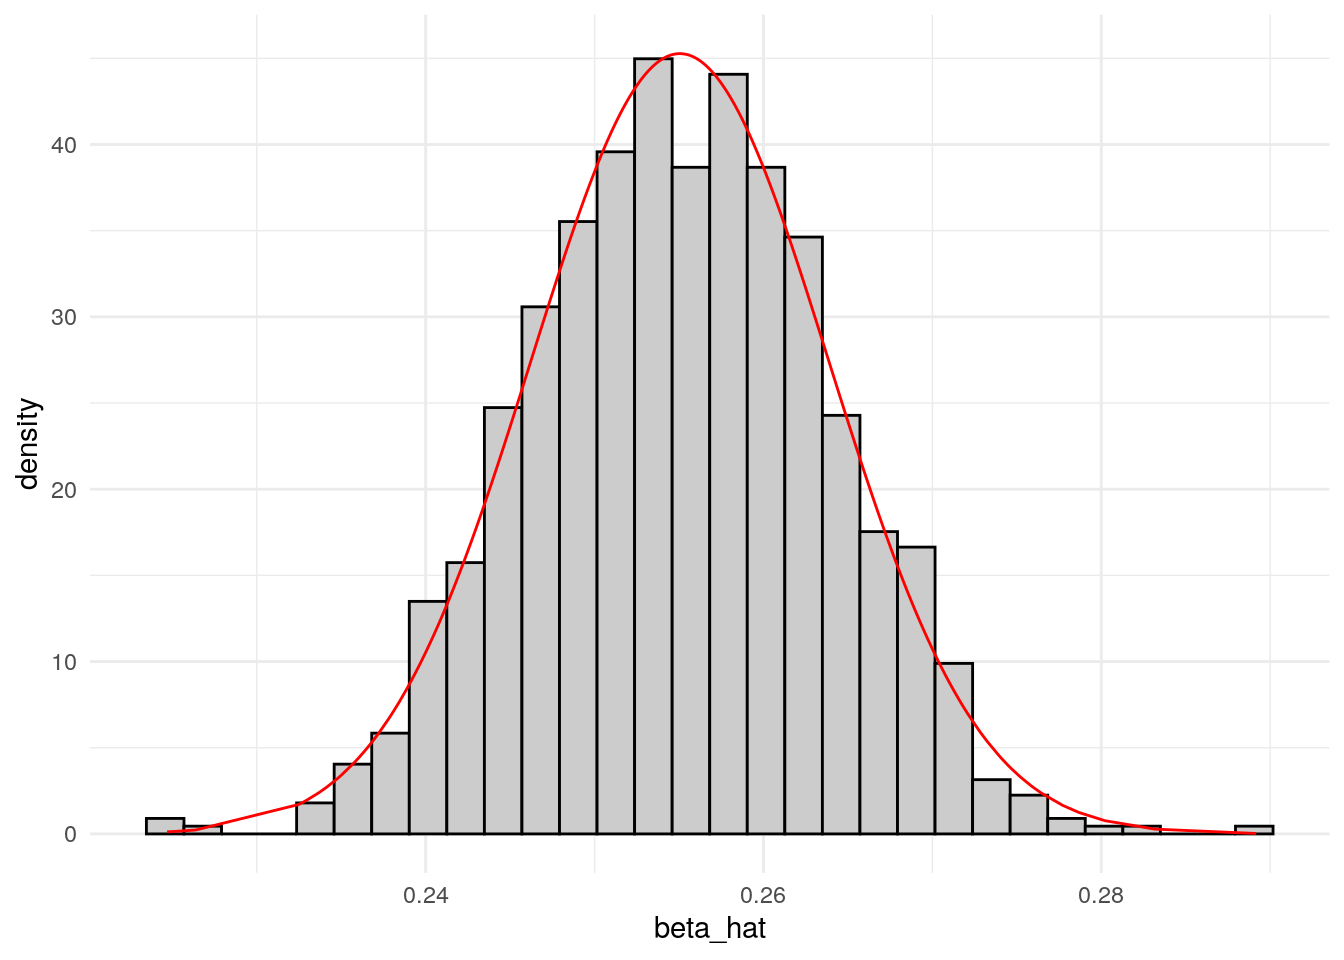
\includegraphics[width=0.8\linewidth]{RecEx8-sol_files/figure-latex/unnamed-chunk-10-1}

\begin{enumerate}
\def\labelenumi{\alph{enumi})}
\setcounter{enumi}{5}
\item
\end{enumerate}

\begin{Shaded}
\begin{Highlighting}[]
\KeywordTok{library}\NormalTok{(gbm)}
\NormalTok{r.boost =}\StringTok{ }\KeywordTok{gbm}\NormalTok{(Sales }\OperatorTok{~}\StringTok{ }\NormalTok{., Carseats.train, }\DataTypeTok{distribution =} \StringTok{"gaussian"}\NormalTok{, }\DataTypeTok{n.trees =} \DecValTok{500}\NormalTok{, }
    \DataTypeTok{interaction.depth =} \DecValTok{4}\NormalTok{, }\DataTypeTok{shrinkage =} \FloatTok{0.1}\NormalTok{)}
\NormalTok{yhat.boost =}\StringTok{ }\KeywordTok{predict}\NormalTok{(r.boost, }\DataTypeTok{newdata =}\NormalTok{ Carseats.test, }\DataTypeTok{n.trees =} \DecValTok{500}\NormalTok{)}
\NormalTok{mse_boost <-}\StringTok{ }\KeywordTok{mean}\NormalTok{((yhat.boost }\OperatorTok{-}\StringTok{ }\NormalTok{Carseats.test}\OperatorTok{$}\NormalTok{Sales)}\OperatorTok{^}\DecValTok{2}\NormalTok{)}
\NormalTok{mse_boost}
\end{Highlighting}
\end{Shaded}

\begin{verbatim}
## [1] 2.151292
\end{verbatim}

We see a further decrease in MSE by boosing our trees.

\begin{enumerate}
\def\labelenumi{\alph{enumi})}
\setcounter{enumi}{6}
\item
\end{enumerate}

\begin{Shaded}
\begin{Highlighting}[]
\NormalTok{train.predictors =}\StringTok{ }\NormalTok{Carseats.train[, }\DecValTok{-1}\NormalTok{]}
\NormalTok{test.predictors =}\StringTok{ }\NormalTok{Carseats.test[, }\DecValTok{-1}\NormalTok{]}
\NormalTok{Y.train =}\StringTok{ }\NormalTok{Carseats.train[, }\DecValTok{1}\NormalTok{]}
\NormalTok{Y.test =}\StringTok{ }\NormalTok{Carseats.test[, }\DecValTok{1}\NormalTok{]}

\NormalTok{bag.Car =}\StringTok{ }\KeywordTok{randomForest}\NormalTok{(train.predictors, }\DataTypeTok{y =}\NormalTok{ Y.train, }\DataTypeTok{xtest =}\NormalTok{ test.predictors, }\DataTypeTok{ytest =}\NormalTok{ Y.test, }
    \DataTypeTok{mtry =} \DecValTok{10}\NormalTok{, }\DataTypeTok{ntree =} \DecValTok{500}\NormalTok{)}
\NormalTok{rf.Car =}\StringTok{ }\KeywordTok{randomForest}\NormalTok{(train.predictors, }\DataTypeTok{y =}\NormalTok{ Y.train, }\DataTypeTok{xtest =}\NormalTok{ test.predictors, }\DataTypeTok{ytest =}\NormalTok{ Y.test, }
    \DataTypeTok{mtry =} \DecValTok{3}\NormalTok{, }\DataTypeTok{ntree =} \DecValTok{500}\NormalTok{)}
\KeywordTok{plot}\NormalTok{(}\DecValTok{1}\OperatorTok{:}\DecValTok{500}\NormalTok{, bag.Car}\OperatorTok{$}\NormalTok{test}\OperatorTok{$}\NormalTok{mse, }\DataTypeTok{col =} \StringTok{"blue"}\NormalTok{, }\DataTypeTok{type =} \StringTok{"l"}\NormalTok{, }\DataTypeTok{xlab =} \StringTok{"Number of Trees"}\NormalTok{, }
    \DataTypeTok{ylab =} \StringTok{"Test MSE"}\NormalTok{, }\DataTypeTok{ylim =} \KeywordTok{c}\NormalTok{(}\DecValTok{2}\NormalTok{, }\FloatTok{2.8}\NormalTok{))}
\KeywordTok{lines}\NormalTok{(}\DecValTok{1}\OperatorTok{:}\DecValTok{500}\NormalTok{, rf.Car}\OperatorTok{$}\NormalTok{test}\OperatorTok{$}\NormalTok{mse, }\DataTypeTok{col =} \StringTok{"green"}\NormalTok{)}

\KeywordTok{legend}\NormalTok{(}\StringTok{"topright"}\NormalTok{, }\KeywordTok{c}\NormalTok{(}\StringTok{"m = p"}\NormalTok{, }\StringTok{"m = p/3"}\NormalTok{), }\DataTypeTok{col =} \KeywordTok{c}\NormalTok{(}\StringTok{"blue"}\NormalTok{, }\StringTok{"green"}\NormalTok{), }\DataTypeTok{cex =} \DecValTok{1}\NormalTok{, }\DataTypeTok{lty =} \DecValTok{1}\NormalTok{)}
\end{Highlighting}
\end{Shaded}

\includegraphics[width=0.7\linewidth]{RecEx8-sol_files/figure-latex/unnamed-chunk-12-1}

\hypertarget{problem-3-classification}{%
\subsection{Problem 3 --
Classification}\label{problem-3-classification}}

\begin{Shaded}
\begin{Highlighting}[]
\KeywordTok{library}\NormalTok{(kernlab)}
\KeywordTok{data}\NormalTok{(spam)}
\end{Highlighting}
\end{Shaded}

\begin{enumerate}
\def\labelenumi{\alph{enumi})}
\item
\end{enumerate}

Do this in R and read the Description.

\begin{enumerate}
\def\labelenumi{\alph{enumi})}
\setcounter{enumi}{1}
\item
\end{enumerate}

\begin{Shaded}
\begin{Highlighting}[]
\KeywordTok{library}\NormalTok{(ISLR)}
\KeywordTok{set.seed}\NormalTok{(}\DecValTok{4268}\NormalTok{)}
\NormalTok{n =}\StringTok{ }\KeywordTok{nrow}\NormalTok{(spam)}
\NormalTok{train =}\StringTok{ }\KeywordTok{sample}\NormalTok{(}\DecValTok{1}\OperatorTok{:}\NormalTok{n, }\FloatTok{0.7} \OperatorTok{*}\StringTok{ }\NormalTok{n, }\DataTypeTok{replace =}\NormalTok{ F)}
\NormalTok{test =}\StringTok{ }\NormalTok{(}\DecValTok{1}\OperatorTok{:}\NormalTok{n)[}\OperatorTok{-}\NormalTok{train]}
\NormalTok{spam.train =}\StringTok{ }\NormalTok{spam[train, ]}
\NormalTok{spam.test =}\StringTok{ }\NormalTok{spam[}\OperatorTok{-}\NormalTok{train, ]}
\end{Highlighting}
\end{Shaded}

\begin{enumerate}
\def\labelenumi{\alph{enumi})}
\setcounter{enumi}{2}
\item
\end{enumerate}

\begin{Shaded}
\begin{Highlighting}[]
\NormalTok{spam.tree =}\StringTok{ }\KeywordTok{tree}\NormalTok{(type }\OperatorTok{~}\StringTok{ }\NormalTok{., spam, }\DataTypeTok{subset =}\NormalTok{ train)}

\KeywordTok{plot}\NormalTok{(spam.tree)}
\KeywordTok{text}\NormalTok{(spam.tree, }\DataTypeTok{pretty =} \DecValTok{1}\NormalTok{)}
\end{Highlighting}
\end{Shaded}

\includegraphics[width=0.7\linewidth]{RecEx8-sol_files/figure-latex/unnamed-chunk-15-1}

\begin{Shaded}
\begin{Highlighting}[]
\KeywordTok{summary}\NormalTok{(spam.tree)}
\end{Highlighting}
\end{Shaded}

\begin{verbatim}
## 
## Classification tree:
## tree(formula = type ~ ., data = spam, subset = train)
## Variables actually used in tree construction:
## [1] "charExclamation" "remove"          "charDollar"      "george"         
## [5] "hp"              "capitalLong"     "our"             "capitalAve"     
## [9] "hpl"            
## Number of terminal nodes:  14 
## Residual mean deviance:  0.4801 = 1539 / 3206 
## Misclassification error rate: 0.08975 = 289 / 3220
\end{verbatim}

\begin{enumerate}
\def\labelenumi{\alph{enumi})}
\setcounter{enumi}{3}
\item
\end{enumerate}

\begin{Shaded}
\begin{Highlighting}[]
\NormalTok{yhat =}\StringTok{ }\KeywordTok{predict}\NormalTok{(spam.tree, spam[test, ], }\DataTypeTok{type =} \StringTok{"class"}\NormalTok{)}
\NormalTok{response.test =}\StringTok{ }\NormalTok{spam}\OperatorTok{$}\NormalTok{type[test]}

\NormalTok{misclass =}\StringTok{ }\KeywordTok{table}\NormalTok{(yhat, response.test)}
\NormalTok{misclass}
\end{Highlighting}
\end{Shaded}

\begin{verbatim}
##          response.test
## yhat      nonspam spam
##   nonspam     781   67
##   spam         67  466
\end{verbatim}

\begin{Shaded}
\begin{Highlighting}[]
\DecValTok{1} \OperatorTok{-}\StringTok{ }\KeywordTok{sum}\NormalTok{(}\KeywordTok{diag}\NormalTok{(misclass))}\OperatorTok{/}\KeywordTok{sum}\NormalTok{(misclass)}
\end{Highlighting}
\end{Shaded}

\begin{verbatim}
## [1] 0.09703114
\end{verbatim}

\begin{enumerate}
\def\labelenumi{\alph{enumi})}
\setcounter{enumi}{4}
\item
\end{enumerate}

\begin{Shaded}
\begin{Highlighting}[]
\KeywordTok{set.seed}\NormalTok{(}\DecValTok{4268}\NormalTok{)}

\NormalTok{cv.spam =}\StringTok{ }\KeywordTok{cv.tree}\NormalTok{(spam.tree, }\DataTypeTok{FUN =}\NormalTok{ prune.misclass)}

\KeywordTok{plot}\NormalTok{(cv.spam}\OperatorTok{$}\NormalTok{size, cv.spam}\OperatorTok{$}\NormalTok{dev, }\DataTypeTok{type =} \StringTok{"b"}\NormalTok{)}
\end{Highlighting}
\end{Shaded}

\includegraphics[width=0.7\linewidth]{RecEx8-sol_files/figure-latex/unnamed-chunk-17-1}

According to the plot the optimal number of terminal nodes is 6 (or
larger). We choose 6 as this gives the simplest tree, and prune the tree
according to this value.

\begin{Shaded}
\begin{Highlighting}[]
\NormalTok{prune.spam =}\StringTok{ }\KeywordTok{prune.misclass}\NormalTok{(spam.tree, }\DataTypeTok{best =} \DecValTok{6}\NormalTok{)}

\KeywordTok{plot}\NormalTok{(prune.spam)}
\KeywordTok{text}\NormalTok{(prune.spam, }\DataTypeTok{pretty =} \DecValTok{1}\NormalTok{)}
\end{Highlighting}
\end{Shaded}

\includegraphics[width=0.7\linewidth]{RecEx8-sol_files/figure-latex/unnamed-chunk-18-1}

We predict the response for the test data:

\begin{Shaded}
\begin{Highlighting}[]
\NormalTok{yhat.prune =}\StringTok{ }\KeywordTok{predict}\NormalTok{(prune.spam, spam[test, ], }\DataTypeTok{type =} \StringTok{"class"}\NormalTok{)}

\NormalTok{misclass.prune =}\StringTok{ }\KeywordTok{table}\NormalTok{(yhat.prune, response.test)}
\NormalTok{misclass.prune}
\end{Highlighting}
\end{Shaded}

\begin{verbatim}
##           response.test
## yhat.prune nonspam spam
##    nonspam     796  104
##    spam         52  429
\end{verbatim}

The misclassification rate is

\begin{Shaded}
\begin{Highlighting}[]
\DecValTok{1} \OperatorTok{-}\StringTok{ }\KeywordTok{sum}\NormalTok{(}\KeywordTok{diag}\NormalTok{(misclass.prune))}\OperatorTok{/}\KeywordTok{sum}\NormalTok{(misclass.prune)}
\end{Highlighting}
\end{Shaded}

\begin{verbatim}
## [1] 0.1129616
\end{verbatim}

\begin{enumerate}
\def\labelenumi{\alph{enumi})}
\setcounter{enumi}{5}
\item
\end{enumerate}

\begin{Shaded}
\begin{Highlighting}[]
\KeywordTok{library}\NormalTok{(randomForest)}
\NormalTok{bag.spam =}\StringTok{ }\KeywordTok{randomForest}\NormalTok{(type }\OperatorTok{~}\StringTok{ }\NormalTok{., }\DataTypeTok{data =}\NormalTok{ spam, }\DataTypeTok{subset =}\NormalTok{ train, }\DataTypeTok{mtry =} \KeywordTok{ncol}\NormalTok{(spam) }\OperatorTok{-}\StringTok{ }
\StringTok{    }\DecValTok{1}\NormalTok{, }\DataTypeTok{ntree =} \DecValTok{500}\NormalTok{, }\DataTypeTok{importance =} \OtherTok{TRUE}\NormalTok{)}
\end{Highlighting}
\end{Shaded}

We predict the response for the test data as before:

\begin{Shaded}
\begin{Highlighting}[]
\NormalTok{yhat.bag =}\StringTok{ }\KeywordTok{predict}\NormalTok{(bag.spam, }\DataTypeTok{newdata =}\NormalTok{ spam[test, ])}

\NormalTok{misclass.bag =}\StringTok{ }\KeywordTok{table}\NormalTok{(yhat.bag, response.test)}
\NormalTok{misclass.bag}
\end{Highlighting}
\end{Shaded}

\begin{verbatim}
##          response.test
## yhat.bag  nonspam spam
##   nonspam     810   43
##   spam         38  490
\end{verbatim}

The misclassification rate is

\begin{Shaded}
\begin{Highlighting}[]
\DecValTok{1} \OperatorTok{-}\StringTok{ }\KeywordTok{sum}\NormalTok{(}\KeywordTok{diag}\NormalTok{(misclass.bag))}\OperatorTok{/}\KeywordTok{sum}\NormalTok{(misclass.bag)}
\end{Highlighting}
\end{Shaded}

\begin{verbatim}
## [1] 0.05865315
\end{verbatim}

\begin{enumerate}
\def\labelenumi{\alph{enumi})}
\setcounter{enumi}{6}
\item
\end{enumerate}

We now use the random forest-algorithm and consider only
\(\sqrt{57}\approx 8\) of the predictors at each split. This is
specified in \texttt{mtry}.

\begin{Shaded}
\begin{Highlighting}[]
\KeywordTok{set.seed}\NormalTok{(}\DecValTok{4268}\NormalTok{)}
\NormalTok{rf.spam =}\StringTok{ }\KeywordTok{randomForest}\NormalTok{(type }\OperatorTok{~}\StringTok{ }\NormalTok{., }\DataTypeTok{data =}\NormalTok{ spam, }\DataTypeTok{subset =}\NormalTok{ train, }\DataTypeTok{mtry =} \KeywordTok{round}\NormalTok{(}\KeywordTok{sqrt}\NormalTok{(}\KeywordTok{ncol}\NormalTok{(spam) }\OperatorTok{-}\StringTok{ }
\StringTok{    }\DecValTok{1}\NormalTok{)), }\DataTypeTok{ntree =} \DecValTok{500}\NormalTok{, }\DataTypeTok{importance =} \OtherTok{TRUE}\NormalTok{)}
\end{Highlighting}
\end{Shaded}

We study the importance of each variable

\begin{Shaded}
\begin{Highlighting}[]
\KeywordTok{importance}\NormalTok{(rf.spam)}
\end{Highlighting}
\end{Shaded}

If \texttt{MeanDecreaseAccuracy} and \texttt{MeanDecreaseGini} are
large, the corresponding covariate is important.

\begin{Shaded}
\begin{Highlighting}[]
\KeywordTok{varImpPlot}\NormalTok{(rf.spam)}
\end{Highlighting}
\end{Shaded}

\includegraphics[width=0.9\linewidth]{RecEx8-sol_files/figure-latex/unnamed-chunk-26-1}

In this plot we see that \texttt{charExclamation} is the most important
covariate, followed by \texttt{remove} and \texttt{charDollar}. This is
as expected as these variables are used in the top splits in the
classification trees we have seen so far.

We now predict the response for the test data.

\begin{Shaded}
\begin{Highlighting}[]
\NormalTok{yhat.rf =}\StringTok{ }\KeywordTok{predict}\NormalTok{(rf.spam, }\DataTypeTok{newdata =}\NormalTok{ spam[test, ])}

\NormalTok{misclass.rf =}\StringTok{ }\KeywordTok{table}\NormalTok{(yhat.rf, response.test)}
\DecValTok{1} \OperatorTok{-}\StringTok{ }\KeywordTok{sum}\NormalTok{(}\KeywordTok{diag}\NormalTok{(misclass.rf))}\OperatorTok{/}\KeywordTok{sum}\NormalTok{(misclass.rf)}
\end{Highlighting}
\end{Shaded}

\begin{verbatim}
## [1] 0.044895
\end{verbatim}

The misclassification rate is given by

\begin{Shaded}
\begin{Highlighting}[]
\NormalTok{misclass.rf}
\end{Highlighting}
\end{Shaded}

\begin{verbatim}
##          response.test
## yhat.rf   nonspam spam
##   nonspam     824   38
##   spam         24  495
\end{verbatim}

\begin{enumerate}
\def\labelenumi{\alph{enumi})}
\setcounter{enumi}{7}
\item
\end{enumerate}

The \texttt{gbm()} function does not allow factors, so we have to use
`1' and `0' instead of \texttt{spam} and \texttt{nonspam}

\begin{Shaded}
\begin{Highlighting}[]
\KeywordTok{library}\NormalTok{(gbm)}
\KeywordTok{set.seed}\NormalTok{(}\DecValTok{4268}\NormalTok{)}

\NormalTok{spamboost =}\StringTok{ }\NormalTok{spam}
\NormalTok{spamboost}\OperatorTok{$}\NormalTok{type =}\StringTok{ }\KeywordTok{c}\NormalTok{()}
\NormalTok{spamboost}\OperatorTok{$}\NormalTok{type[spam}\OperatorTok{$}\NormalTok{type }\OperatorTok{==}\StringTok{ "spam"}\NormalTok{] =}\StringTok{ }\DecValTok{1}
\NormalTok{spamboost}\OperatorTok{$}\NormalTok{type[spam}\OperatorTok{$}\NormalTok{type }\OperatorTok{==}\StringTok{ "nonspam"}\NormalTok{] =}\StringTok{ }\DecValTok{0}

\NormalTok{boost.spam =}\StringTok{ }\KeywordTok{gbm}\NormalTok{(type }\OperatorTok{~}\StringTok{ }\NormalTok{., }\DataTypeTok{data =}\NormalTok{ spamboost[train, ], }\DataTypeTok{distribution =} \StringTok{"bernoulli"}\NormalTok{, }
    \DataTypeTok{n.trees =} \DecValTok{5000}\NormalTok{, }\DataTypeTok{interaction.depth =} \DecValTok{3}\NormalTok{, }\DataTypeTok{shrinkage =} \FloatTok{0.001}\NormalTok{)}
\end{Highlighting}
\end{Shaded}

We predict the response for the test data

\begin{Shaded}
\begin{Highlighting}[]
\NormalTok{yhat.boost =}\StringTok{ }\KeywordTok{predict}\NormalTok{(boost.spam, }\DataTypeTok{newdata =}\NormalTok{ spamboost[}\OperatorTok{-}\NormalTok{train, ], }\DataTypeTok{n.trees =} \DecValTok{5000}\NormalTok{, }\DataTypeTok{distribution =} \StringTok{"bernoulli"}\NormalTok{, }
    \DataTypeTok{type =} \StringTok{"response"}\NormalTok{)}

\NormalTok{yhat.boost =}\StringTok{ }\KeywordTok{ifelse}\NormalTok{(yhat.boost }\OperatorTok{>}\StringTok{ }\FloatTok{0.5}\NormalTok{, }\DecValTok{1}\NormalTok{, }\DecValTok{0}\NormalTok{)  }\CommentTok{#Transform to 0 and 1 (nonspam and spam).}

\NormalTok{misclass.boost =}\StringTok{ }\KeywordTok{table}\NormalTok{(yhat.boost, spamboost}\OperatorTok{$}\NormalTok{type[test])}

\NormalTok{misclass.boost}
\end{Highlighting}
\end{Shaded}

\begin{verbatim}
##           
## yhat.boost   0   1
##          0 812  52
##          1  36 481
\end{verbatim}

and the misclassification rate is

\begin{Shaded}
\begin{Highlighting}[]
\DecValTok{1} \OperatorTok{-}\StringTok{ }\KeywordTok{sum}\NormalTok{(}\KeywordTok{diag}\NormalTok{(misclass.boost))}\OperatorTok{/}\KeywordTok{sum}\NormalTok{(misclass.boost)}
\end{Highlighting}
\end{Shaded}

\begin{verbatim}
## [1] 0.06372194
\end{verbatim}

\begin{enumerate}
\def\labelenumi{\roman{enumi})}
\item
\end{enumerate}

We get lower missclassification rates for bagging, random forest and
boosting than for a simple tree, which is expected.

\end{document}
